\section{実験} \label{sec:Experiments}

実験の目的は、提案手法のレーティング予測における優位性と、
提案手法に反映されている意図が実際にレーティング予測において有効であるかの
検証である。
具体的には、提案手法が従来手法\cite{fujitani15}に対して
優れているかを検証する。
また、提案手法を単純にした複数の比較手法を用意し、
提案手法がそれらより有意に優れていることを示す。
さらに、提案手法と比較手法及び比較手法同士の比較により、
文同士の位置関係の考慮や文書ベクトルと文ベクトルを同時に用いることが
レーティング予測に有効であるかを検証する。


\subsection{実験設定}

実験には、正答率を測定する実験と
提案手法における予測レーティングと正解レーティングのRMSEを
測定する実験の2つを行った。
比較手法として、提案手法における分類器の入力をそれぞれ
(1) DV (Document Vector)、
(2) ASV (Averaged Sentence Vector)、
(3) Weighted ASV
に変えた手法を用意した。
DVとはレビュー全体の文書ベクトルであり、
Quocら\cite{quoc14}の手法に相当する。
ASVとはレビュー内で平均した文ベクトルであり、
Weighted ASVとはレビュー内で重み付け平均によって圧縮された文ベクトルである。
Weighted ASVにおいて重み付け平均の方法は提案手法と同様であるが、
重み付け平均の式のハイパーパラメータは別に調整した。
有意差検定にはマクネマー検定を用い、p値が0.05より小さいとき有意とした。
また、RMSEの計算において正解または予測レーティングが0点であるものは
評価から省いた。
これは用いるデータセットのレビューにおいて、レーティングの0点は
レーティングが不可能であることを意味するためである。

データセットとしては、先行研究\cite{fujitani15}と同様に、
ホテル予約サイト楽天トラベルにおけるレビュー337,266件からレビューの番号順に
訓練データ300,000件、開発データ10,000件、評価データ10,000件を用いた。
楽天トラベルによって提供されている元のレビューデータは
レーティングを含むファイルとレビューの文書を含むファイルとに分かれている。
それぞれTab Separated Values (TSV)フォーマットで1行1レビューとして情報が
記述されている。
レーティングを含むファイルと文書を含むファイルのフォーマットを
それぞれ図\ref{fig:RatingFileFormat}と図\ref{fig:DocumentFileFormat}に示す。
以下に、それぞれのファイルから実験のために抽出した情報と
それらの前処理について記述する。
まず、レーティングを含むファイルからは、レビューのIDと
「立地」から「総合」カテゴリまでのレーティングを取り出した。
レビューの文書を含むファイルからは、レビューのIDと
レビューの文書を取り出した。
ただし、元のレビューの文書に含まれる「【ご利用の宿泊プラン】」以降の文字列は
ユーザが記述したものではないため取り除いた。
その後、レーティングとレビューの文書をレビューIDが一致するように組にした。
このとき、レーティングを含むファイル、または、レビューの文書を含むファイルの
どちらかにしか存在しないレビューIDを持つレビューは取り除いた。

\begin{figure}
  第1フィールド(レビューのID){[Tab]}第2フィールド{[Tab]} ... \\
  第7フィールド(「立地」カテゴリのレーティング){[Tab]} ... \\
  第13フィールド(「総合」カテゴリのレーティング)
  \caption{レーティングを含むTSVファイルのフォーマット}
  \label{fig:RatingFileFormat}
\end{figure}

\begin{figure}
  第1フィールド{[Tab]}第2フィールド(レビューの文書){[Tab]} \\
  第3フィールド(レビューのID){[Tab]} ...
  \caption{文書を含むTSVファイルのフォーマット}
  \label{fig:DocumentFileFormat}
\end{figure}

レビューの文書に対する前処理について以下に示す。
まず、全てのレビューの文書に対して文字コードをUTF-8に変換し、
以下の正規化処理を行った。
記号「!”#$%&’()*+,−./:;<>?@[¥]^_`{|}
\unicode{301C}」は全てNFKC形式で正規化した。
記号「\unicode{02D7}\unicode{058A}\unicode{2011}\unicode{2012}\unicode{2013}
\unicode{2043}\unicode{207B}\unicode{208B}\unicode{2212}」
は全て記号「-」で置き換えた。
記号「\unicode{FE63}-ー—―─━ー」は全て記号「ー」で置き換えた。
チルダ記号「\unicode{007E}\unicode{223C}\unicode{223E}\unicode{301C}
\unicode{3030}\unicode{FF5E}」は全て削除した。
ここで、\unicode{XXXX}は16進数で表現されたUnicodeのコードポイントを示す。
次に、各レビューの文書を文に分割した。
「。」、「.」、「!」、「?」を文の終端文字とし、
文の終端文字でない文字の1回より多い繰り返しと
文の終端文字または文書の終端の連続を
一つの文として正規表現によって解析した。
ただし、文が1つも解析できなかった文書については、
文書全体の文字列をその文書に含まれる唯一の文とした。
最後に、形態素解析には形態素解析器MeCabを用いた、
辞書にはIPA辞書を用いた。
単語の情報は表層のみを利用し、MeCabによって出力される
表層が無い特殊な単語は取り除いた。

表\ref{tab:ParametersOfMethods}に各手法におけるニューラルネットワークの
パラメータ設定を示す。
全ての手法において、中間層の数は1、入力層及び中間層におけるドロップアウト率は
それぞれ0.2と0.5で共通である。
Adam\cite{diederik15}のハイパーパラメータは\cite{diederik15}と同様の値を
用いた。
Weighted ASVと提案手法において圧縮された文ベクトルの数は
それぞれ3つと2つとした。
全ての実験において文書及び文ベクトルについては、
学習回数は1,024回、学習する単語の範囲は前3単語、単語の最少出現回数は5回、
ネガティブサンプリングの回数は5回、ベクトルの次元数は600次元に
設定し学習したものを用いた。

\begin{table}
  \caption{各手法のパラメータ設定}
  \centering
  \begin{tabular}{l | r r} \label{tab:ParametersOfMethods}
    手法 & 学習回数 & 中間層でのユニット数 \\
    \hline
    DV & 20 & 512 \\
    ASV & 55 & 256 \\
    Weighted ASV & 24 & 256 \\
    提案手法 & 30 & 512 \\
  \end{tabular}
\end{table}


\subsection{結果}

まず、提案手法と3つの比較手法、従来手法\cite{fujitani15}を
正答率で比較したものを表\ref{tab:AccuraciesOfMethods}に示す。
そのグラフを図\ref{fig:AccuraciesOfMethods}に示す。
また、表\ref{tab:AccuraciesPerCategory}に提案手法と
従来手法\cite{fujitani15}におけるカテゴリ別の正答率を示す。
そのグラフを図\ref{tab:AccuraciesPerCategory}に示す。
表\ref{tab:AccuraciesOfMethods}において、
提案手法が従来手法\cite{fujitani15}の正答率を0.0198有意に上回っている。
また、提案手法がDVとWeighted ASVの正答率をそれぞれ0.0050と0.0163
有意に上回っている。
Weighted ASVがASVを0.0029有意に上回っている。

\begin{table}
  \caption{各手法における正答率}
  \centering
  \begin{tabular}{l | r} \label{tab:AccuraciesOfMethods}
    手法 & 正答率 \\
    \hline
    従来手法\cite{fujitani15} & 0.4832 \\
    DV & 0.4980 \\
    ASV & 0.4838 \\
    Weighted ASV & 0.4867 \\
    提案手法 & \textbf{0.5030} \\
  \end{tabular}
\end{table}

\begin{figure}
  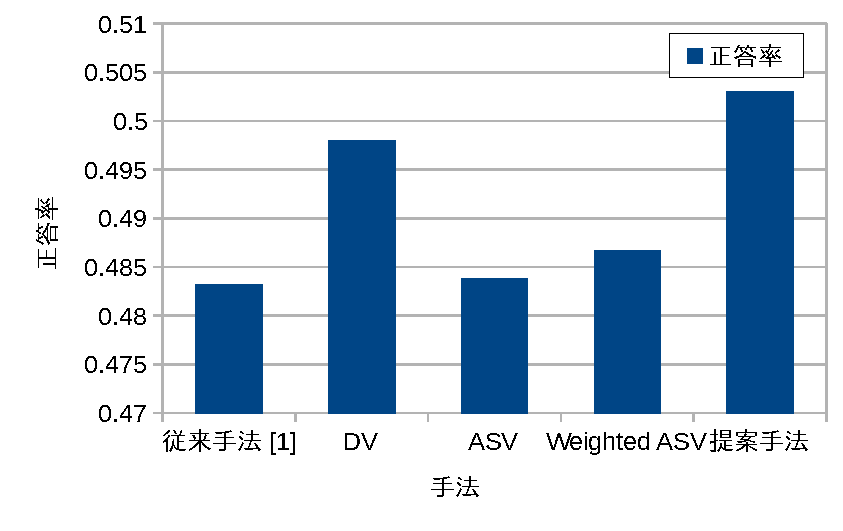
\includegraphics{fig/graph_of_accuracies_of_methods.pdf}
  \caption{各手法における正答率}
  \label{fig:AccuraciesOfMethods}
\end{figure}

\begin{table}
  \caption{提案手法と従来手法\cite{fujitani15}におけるカテゴリ別の正答率}
  \centering
  \begin{tabular}{r | r r r r r r r} \label{tab:AccuraciesPerCategory}
    手法 & 立地 & 部屋 & 食事 & 風呂 & サービス & 設備 & 総合 \\
    \hline
    従来手法\cite{fujitani15}
        & 0.4961 & 0.4706 & 0.5140 & 0.3973 & 0.4783 & 0.4265 & 0.5660 \\
    提案手法 & 0.5140 & 0.4984 & 0.5353 & 0.4347 & 0.5116 & 0.4479 & 0.5794 \\
  \end{tabular}
\end{table}

\begin{figure}
  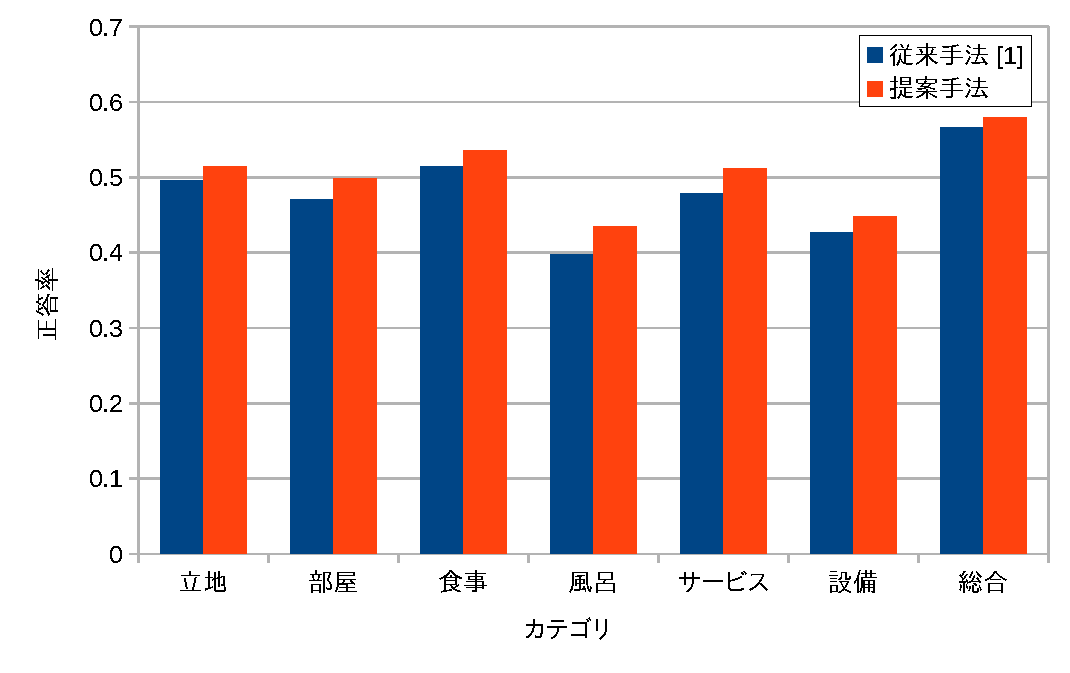
\includegraphics{fig/graph_of_accuracies_per_category.pdf}
  \caption{提案手法と従来手法\cite{fujitani15}におけるカテゴリ別の正答率}
  \label{fig:AccuraciesPerCategory}
\end{figure}

次に、表\ref{tab:RMSEsPerCategory}にレーティングのRMSEを測定した結果を示す。
そのグラフを図\ref{tab:RMSEsPerCategory}に示す。
提案手法は従来手法\cite{fujitani15}が欠点としていた
食事と風呂のカテゴリにおいてそれぞれ0.65及び0.34だけ低い誤差を示した。
また、その他全てのカテゴリにおいても提案手法は従来手法より低い誤差を示した。

\begin{table}
  \caption{提案手法と従来手法\cite{fujitani15}におけるカテゴリ別の
           レーティングのRMSE}
  \centering
  \begin{tabular}{r | r r r r r r r} \label{tab:RMSEsPerCategory}
    手法 & 立地 & 部屋 & 食事 & 風呂 & サービス & 設備 & 総合 \\
    \hline
    従来手法\cite{fujitani15}
        & 0.97 & 0.97 & 1.53 & 1.27 & 0.94 & 0.95 & 0.81 \\
    提案手法 & 0.88 & 0.88 & 0.93 & 1.03 & 0.86 & 0.90 & 0.73 \\
  \end{tabular}
\end{table}

\begin{figure}
  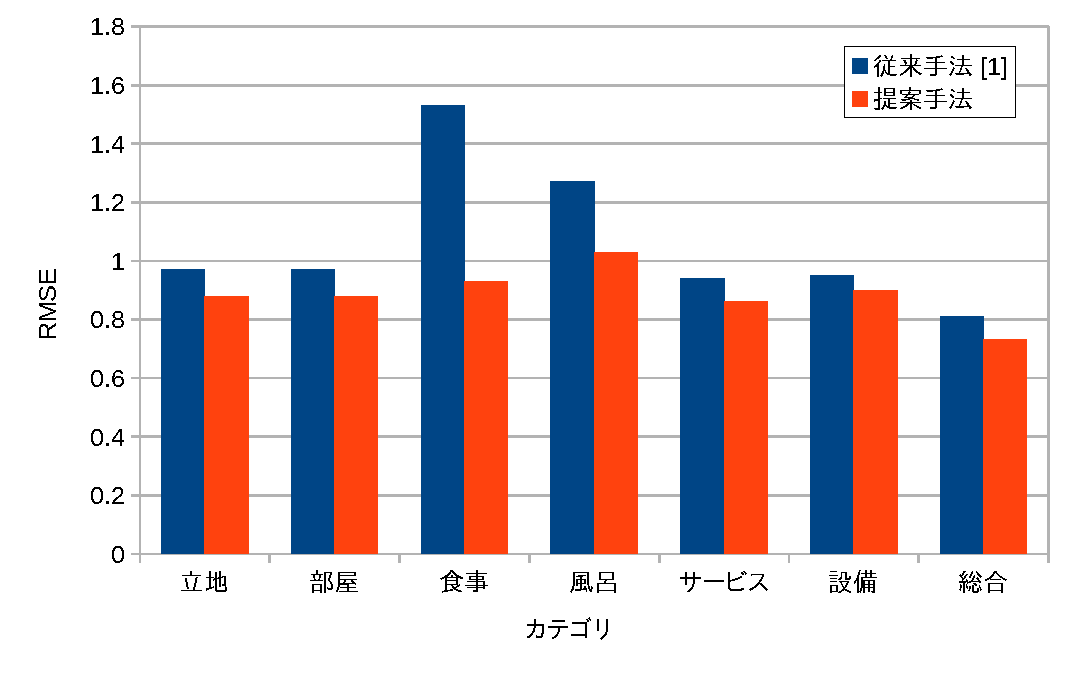
\includegraphics{fig/graph_of_rmses_per_category.pdf}
  \caption{提案手法と従来手法\cite{fujitani15}におけるカテゴリ別の
           レーティングのRMSE}
  \label{fig:RMSEsPerCategory}
\end{figure}

最後に、正答率を測定する実験における、提案手法の精度と再現率、F値を
それぞれ表\ref{tab:ProposedMethodPrecision}と
表\ref{tab:ProposedMethodRecall}、表\ref{tab:ProposedMethodFValue}に示す。
表においてN/Aは計算不可能であることを示す。
また、カテゴリ毎の正解レーティングの内訳と
提案手法のカテゴリ毎の予測レーティングの内訳を
表\ref{tab:AnswerRatings}と表\ref{tab:PredictedRatings}に示す。

\begin{table}
  \caption{提案手法の精度}
  \centering
  \begin{tabular}{r | r r r r r r r | r} \label{tab:ProposedMethodPrecision}
    レーティング & 立地 & 部屋 & 食事 & 風呂 & サービス & 設備 & 総合
      & 全カテゴリ \\
    \hline
    \csvreader[no head,late after line=\\]
      {csv/class_precision.csv}
      {1=\rating,2=\location,3=\room,4=\mean,5=\bath,6=\service,7=\facilities,
       8=\overall,9=\allcategories}
      {\rating & \location & \room & \mean & \bath & \service & \facilities
       & \overall & \allcategories}
  \end{tabular}
\end{table}

\begin{table}
  \caption{提案手法の再現率}
  \centering
  \begin{tabular}{r | r r r r r r r | r} \label{tab:ProposedMethodRecall}
    レーティング & 立地 & 部屋 & 食事 & 風呂 & サービス & 設備 & 総合
      & 全カテゴリ \\
    \hline
    \csvreader[no head,late after line=\\]
      {csv/class_recall.csv}
      {1=\rating,2=\location,3=\room,4=\mean,5=\bath,6=\service,7=\facilities,
       8=\overall,9=\allcategories}
      {\rating & \location & \room & \mean & \bath & \service & \facilities
       & \overall & \allcategories}
  \end{tabular}
\end{table}

\begin{table}
  \caption{提案手法のF値}
  \centering
  \begin{tabular}{r | r r r r r r r | r} \label{tab:ProposedMethodFValue}
    レーティング & 立地 & 部屋 & 食事 & 風呂 & サービス & 設備 & 総合
      & 全カテゴリ \\
    \hline
    \csvreader[no head,late after line=\\]
      {csv/class_f_value.csv}
      {1=\rating,2=\location,3=\room,4=\mean,5=\bath,6=\service,7=\facilities,
       8=\overall,9=\allcategories}
      {\rating & \location & \room & \mean & \bath & \service & \facilities
       & \overall & \allcategories}
  \end{tabular}
\end{table}

\begin{table}
  \caption{カテゴリ毎の正解レーティング件数}
  \centering
  \begin{tabular}{r | r r r r r r r | r} \label{tab:AnswerRatings}
    レーティング & 立地 & 部屋 & 食事 & 風呂 & サービス & 設備 & 総合
      & 全カテゴリ \\
    \hline
    \csvreader[no head,late after line=\\]
      {csv/answer_class_count.csv}
      {1=\rating,2=\location,3=\room,4=\mean,5=\bath,6=\service,7=\facilities,
       8=\overall,9=\allcategories}
      {\rating & \location & \room & \mean & \bath & \service & \facilities
       & \overall & \allcategories}
  \end{tabular}
\end{table}

\begin{table}
  \caption{提案手法のカテゴリ毎の予測レーティング件数}
  \centering
  \begin{tabular}{r | r r r r r r r | r} \label{tab:PredictedRatings}
    レーティング & 立地 & 部屋 & 食事 & 風呂 & サービス & 設備 & 総合
      & 全カテゴリ \\
    \hline
    \csvreader[no head,late after line=\\]
      {csv/predicted_class_count.csv}
      {1=\rating,2=\location,3=\room,4=\mean,5=\bath,6=\service,7=\facilities,
       8=\overall,9=\allcategories}
      {\rating & \location & \room & \mean & \bath & \service & \facilities
       & \overall & \allcategories}
  \end{tabular}
\end{table}
